\documentclass{article}

\usepackage{amsmath}
\usepackage{amssymb}
\usepackage{parskip}
\usepackage{fullpage}
\usepackage{hyperref}
\usepackage{tikz}
\usepackage{bettelini}

\usetikzlibrary{ % tikz packages
    automata,positioning,
    arrows.meta,bending
}

\hypersetup{
    colorlinks=true,
    linkcolor=black,
    urlcolor=blue,
    pdftitle={TheoryOfComputation},
    pdfpagemode=FullScreen,
}

\tikzset{every state/.style={
    inner sep=2pt,
    minimum size=4pt
}}
\tikzset{>=stealth}  %latex, to, stealth

\title{Theory of Computation}
\author{Paolo Bettelini}
\date{}

% Empty string symbol.
\newcommand{\emptyString}{\lambda}

\begin{document}

\maketitle
\tableofcontents
\pagebreak

\section{Fields of Study}

\subsection{Complexity Theory}

Classify problems according to their degree
of "difficulty".

\subsection{Computability Theory}

Classify problems as being solvable or unsolvable.

\subsection{Automata Theory}

Compare different computation models.

\section{Alphabets and Languages}

An \textit{alphabet} is a finite set of \textit{symbols}.
For example: \(\{a,b,c,\cdots, z\}\)\\
The set \(\{0,1\}\) is the binary set.
The empty string is denoted \(\emptyString\).
\\
Note that \(\emptyString \neq \varnothing \neq \{\emptyString\}\).
\\
The length of a string \(w\) is denoted as \(|w|\).

A set of strings is called a \textit{language}.

\section{Deterministic Finite Automaton}

A deterministic finite automaton (DFA) is a state-machine which processes a string
symbol by symbol from left to right. The automaton is in one of his \textit{states}
after processing a symbol. The machine might terminate in an
\textit{accept state} or not.

A DFA \(M=(Q, \Sigma, \delta, q, F)\)
\begin{itemize}
    \item \(Q\) is a finite set of \textit{states}
    \item \(\Sigma\) is an alphabet
    \item \(\delta : Q \times \Sigma \to Q\) is the \textit{transition function}
    \item \(q\) is an element of \(Q\) called the \textit{start state}
    \item \(F\) is a subset of \(Q\) which contains the \textit{accept states}
\end{itemize}
The transition function is the logical components, it determines
in which state the machine will be after processing a symbol at any state.

The following automaton processes a binary string.
The start state is \(q_1\) and the only accept state is \(q_3\).
The program moves to the next state only if the symbol is \(1\),
so it will reach \(q_3\) only if the input string contains at least two \(1\)s.
\begin{center}
    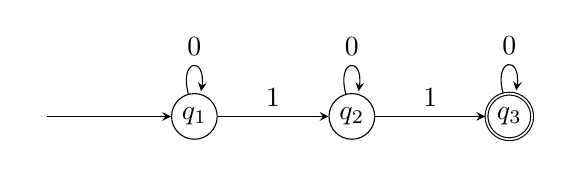
\begin{tikzpicture}[node distance=2cm,on grid,auto]
        \node[state] (q1) {\(q_1\)};
        \node (inv) [left=of q1] {};

        \node[state] (q2) [right=of q1] {\(q_2\)};
        \node[state, accepting] (q3) [right=of q2] {\(q_3\)};

        \path[->]
            (inv)
                edge node {} (q1)
            (q1)
                edge node {\(1\)} (q2)
                edge[loop above] node {\(0\)} ()
            (q2)
                edge node {\(1\)} (q3)
                edge[loop above] node {\(0\)} ()
            (q3)
                edge[loop above] node {\(0\)} ();
    \end{tikzpicture}
\end{center}


If a DFA is in a state \(r\) and it reads the symbol \(a\),
then it will uniquely switch to the state \(\delta(r, a)\)

\pagebreak

The language of \(M\), denoted \(L(M)\) is the set of all accepted strings
by \(M\).

\section{Regular Operations}

\subsection{Union}

If \(A\) and \(B\) are two languages over the same alphabet,
the union of \(A\) and \(B\) is defined as
\[
    A \union B = \{w \suchthat w \in A \lor w \in B\}
\]

\subsection{Concatenation}

If \(A\) and \(B\) are two languages over the same alphabet,
the concatenation of \(A\) and \(B\) is defined as
\[
    AB = \{ab \suchthat a \in A \land b \in B\}
\]

\subsection{Kleene star operator}

The kleene star operator can be applied to alphabets or languages.
It represent the union of all \(n\)-permutations of the set. \\
The set \(\{0,1\}^*\) is the set of
all binary strings. If \(\Sigma\) is an alphabet, \(\Sigma^*\) is the set
of all strings over \(\Sigma\)
\[
    \Sigma^* = \emptyString \cup \bigcup_{n\in\mathbb{N}} \Sigma^n
\]

\subsection{Regular language}

A language is regular if it can be expressed as a regular expression,
or if an automaton that accepts said language exists.

\subsubsection{Closure under union}

\textit{If \(A\) and \(B\) are two regular languages over the same alphabet
\(\Sigma\), there \(A \union B\) is also regular.}

We can prove this by making an automaton that accepts both languages.
Let's say that \(M_1=(Q_1, \Sigma, \delta_1, q_1, F_1)\) accepts \(A\)
and \(M_2=(Q_2, \Sigma, \delta_2, q_2, F_2)\) accepts \(B\).
The automaton \(M=(Q, \Sigma, \delta, q, F)\) must run \(M_1\) and \(M_2\) \textit{simultaneously},
so any state must represent the current states of \(M_1\) and \(M_2\).
This means that the states of \(M\) must represent any combination of state between
\(M_1\) and \(M_2\), meaning \(Q=Q_1 \times Q_2\).
The transition function is now in the form
\(\delta((r_1, r_2), a) = (\delta_1(r_1, a), \delta_2(r_2, a))\) where \(a\in\Sigma\).
The initial state is the state in \(Q\) which contains the initial state of \(M_1\)
and \(M_2\), namely \((q_1, q_2)\). Finally, the set of accept states
is every tuple in \(Q_1\) containing a state in \(F_2\) or in \(Q_2\) containing a state in \(F_1\), namely
\(Q_1 \times F_2 \union Q_2 \times F_1\). \\
We can conclude that \(M=(Q_1 \times Q_2, \Sigma, \delta((r_1, r_2), a), (q_1, q_2), Q_1 \times F_2 \union Q_2 \times F_1)\)
accepts \(A \union B\) so \(A \union B\) is regular.

\pagebreak

\section{Nondeterministic Finite Automaton}

Nondeterministic finite automaton (NFA) are state-machines
like DFAs but can change multiple states at a time by processing
empty strings \(\emptyString\) and when processing a symbol
\(a\) may have multiple possible states to switch to.

\newcommand\double[3][10]{%
  \draw (#2)
    edge [bend left=#1,draw=none]
    coordinate[at start](#2-#3-s)
    coordinate[at end](#2-#3-e)
    (#3)
    edge [bend right=#1,draw=none]
    coordinate[at start](#3-#2-e)
    coordinate[at end](#3-#2-s)
    (#3);
}

\begin{center}
    \begin{tikzpicture}[node distance=2cm,on grid,auto]
        \node[state] (0) {};
        \node (inv) [left=of 0] {};

        \node[state, accepting] (a1) [above right=of 0] {\(q_{a1}\)};
        \node[state] (a2) [right=of a1] {\(q_{a2}\)};
        
        \node[state, accepting] (b1) [below right=of 0] {\(q_{b1}\)};
        \node[state] (b2) [right=of b1] {\(q_{b2}\)};
        \node[state] (b3) [below=of b2] {\(q_{b3}\)};
        
        \double{a1}{a2};

        \path[->]
            (inv)
                edge node {} (0)
            (0)
                edge node {\(\emptyString\)} (a1)
                edge node {\(\emptyString\)} (b1)
            (a1-a2-s)
                edge node {\(1\)} (a1-a2-e)
            (a2-a1-s)
                edge node {\(1\)} (a2-a1-e)
            (b1)
                edge node {\(1\)} (b2)
            (b2)
                edge node {\(1\)} (b3)
            (b3)
                edge node {\(1\)} (b1);
    \end{tikzpicture}
\end{center}

\end{document}

% https://cglab.ca/~michiel/TheoryOfComputation/TheoryOfComputation.pdf
% todo: proofs
% pag 46